\documentclass[12pt,a4paper]{report}

\usepackage[T1]{fontenc}
\usepackage[utf8]{inputenc}
\usepackage[french]{babel}

\usepackage[top=2.5cm,bottom=2.5cm,left=3cm,right=2.5cm]{geometry}

\usepackage{lmodern}
\usepackage{graphicx}
\usepackage{setspace}
\usepackage{fancyhdr}
\usepackage{titlesec}
\usepackage[dvipsnames]{xcolor}
\usepackage{graphicx}
\usepackage{booktabs}
\usepackage{tabularx}
\usepackage{array}
\usepackage{tcolorbox}
\tcbuselibrary{skins}
\usepackage{enumitem}
\usepackage[hidelinks]{hyperref}
\usepackage{microtype}
\usepackage{parskip}

\definecolor{bleu}{RGB}{0,70,140}
\definecolor{grisc}{RGB}{245,245,245}

\onehalfspacing
\setlength{\parindent}{0pt}
\setlength{\parskip}{5pt}

\pagestyle{fancy}
\setlength{\headheight}{14pt}
\fancyhf{}
\fancyhead[L]{\small\textit{TP INGWEB L3 25/26}}
\fancyhead[R]{\small\textit{GROUP 10}}
\fancyfoot[C]{\thepage}
\renewcommand{\headrulewidth}{0.4pt}

\titleformat{\chapter}[block]
  {\normalfont\Large\bfseries\color{bleu}}
  {\thechapter.}{0.8em}{}[\vspace{-0.3em}\rule{\textwidth}{0.4pt}]
\titlespacing*{\chapter}{0pt}{10pt}{15pt}
\titleformat{\section}{\normalfont\large\bfseries\color{bleu}}{\thesection}{0.8em}{}
\titleformat{\subsection}{\normalfont\normalsize\bfseries}{\thesubsection}{0.8em}{}

\newcommand{\HRule}{\rule{\linewidth}{0.5mm}}

\begin{document}

%% ============================================================
%%  PAGE DE GARDE
%% ============================================================

%% ============================================================
%%  TABLE DES MATIERES
%% ============================================================
\tableofcontents
\thispagestyle{fancy}

%% ============================================================
%%  CHAPITRE 1 -- INTRODUCTION
%% ============================================================
\chapter{Introduction g\'en\'erale}

\section{Contexte du projet}

L'enseignement sup\'erieur au cameroun  fait face \`a un
d\'efi constant : concilier la croissance des effectifs estudiantins
avec la disponibilit\'e et la bonne gestion des ressources mat\'erielles.
Au sein du \textbf{D\'epartement de Math\'ematiques et Informatique de
l'Universit\'e de Ngaound\'er\'e}, les enseignants et le personnel
administratif jonglent quotidiennement avec un parc de mat\'eriels
p\'edagogiques vari\'es : projecteurs, capteurs \'electroniques,
marqueurs, \'equipements de travaux pratiques et bien d'autres ressources
partag\'ees entre de nombreuses activit\'es d'enseignement et de recherche.

Dans ce contexte, la gestion manuelle de ces \'equipements se r\'ev\`ele
rapidement insuffisante. Les r\'eservations sont enregistr\'ees sur papier
ou par simple \'echange verbal, les conflits de disponibilit\'e sont
fr\'equents, et le suivi des pr\^ets reste approximatif. Cette situation
g\'en\`ere des pertes de temps, des frustrations chez le corps enseignant,
et des risques de d\'et\'erioration ou de perte du mat\'eriel, faute
de tra\c{c}abilit\'e.

\section{Probl\`eme identifi\'e}

La probl\'ematique centrale de ce projet peut se r\'esumer ainsi :
\textit{comment permettre aux enseignants de r\'eserver facilement le
mat\'eriel p\'edagogique dont ils ont besoin, tout en donnant \`a
l'administration un contr\^ole total sur les stocks, les disponibilit\'es
et l'historique des utilisations~?}

En l'absence d'un outil num\'erique d\'edi\'e, plusieurs
dysfonctionnements sont observ\'es :
\begin{itemize}[noitemsep,topsep=2pt]
  \item des conflits de r\'eservation entre enseignants pour le m\^eme \'equipement ;
  \item une absence de visibilit\'e sur l'\'etat r\'eel du mat\'eriel
        (disponible, en panne, en cours d'utilisation) ;
  \item une tra\c{c}abilit\'e nulle des pr\^ets et des retours, rendant
        impossible l'identification des responsabilit\'es en cas de perte
        ou d'endommagement ;
  \item une charge administrative importante li\'ee \`a la gestion manuelle
        des demandes.
\end{itemize}

\section{Importance et justification du projet}

La digitalisation de la gestion du mat\'eriel p\'edagogique repr\'esente
un enjeu strat\'egique pour le d\'epartement. Un tel outil permettrait
non seulement de fluidifier les processus administratifs, mais aussi
d'am\'eliorer la qualit\'e des enseignements en garantissant que chaque
enseignant dispose du mat\'eriel n\'ecessaire au bon moment. De plus,
en assurant une meilleure tra\c{c}abilit\'e des \'equipements,
l'application contribuerait \`a prolonger leur dur\'ee de vie et \`a
rationaliser les d\'epenses d'acquisition.


\section{Objectif g\'en\'eral du projet}

L'objectif g\'en\'eral de ce projet est de concevoir et de d\'evelopper
une \textbf{application web s\'ecuris\'ee et intuitive} permettant la
gestion compl\`ete du cycle de vie du mat\'eriel p\'edagogique au sein
du D\'epartement de Math\'ematiques et Informatique de l'Universit\'e
de Ngaound\'er\'e : de l'inventaire \`a la r\'eservation, en passant
par la validation administrative, le suivi des pr\^ets et l'analyse
statistique des usages.

%% ============================================================
%%  CHAPITRE 2 -- PRÉSENTATION GÉNÉRALE
%% ============================================================
\chapter{Pr\'esentation g\'en\'erale du projet}

\section{Nom et domaine du projet}

Le projet porte le nom de \textbf{GestMat}
(\textit{Gestionnaire de Mat\'eriel }). Il s'inscrit dans le domaine de
l'\textbf{ing\'enierie des applications web},. Il mobilise des comp\'etences en d\'eveloppement
backend (architecture API REST), en d\'eveloppement frontend (interfaces
utilisateur r\'eactives), en mod\'elisation de bases de donn\'ees
relationnelles, ainsi qu'en s\'ecurit\'e informatique.

\section{Public cible}

L'application est destin\'ee \`a deux cat\'egories d'utilisateurs :

\begin{itemize}
  \item \textbf{Les enseignants :} ils constituent le profil le plus
        nombreux. Leur r\^ole dans l'application se limite \`a consulter
        le catalogue de mat\'eriels disponibles, soumettre des demandes
        de r\'eservation et suivre l'\'etat de leurs demandes.
  \item \textbf{Les administrateurs :} g\'en\'eralement le responsable
        du d\'epartement ou un gestionnaire d\'esign\'e. Ils disposent
        d'un acc\`es complet : gestion des comptes enseignants, validation
        ou rejet des r\'eservations, gestion des stocks, enregistrement
        des pr\^ets et consultation des statistiques d'utilisation.
\end{itemize}

\section{Fonctionnement global de l'application}

L'application suit une architecture client-serveur avec une
\textbf{API REST s\'ecuris\'ee} c\^ot\'e serveur et une
\textbf{interface web dynamique} c\^ot\'e client.
Le flux g\'en\'eral d'utilisation se d\'eroule comme suit :

\begin{enumerate}
  \item Un enseignant se connecte via son identifiant et son mot de passe.
        Un token d'acc\`es s\'ecuris\'e lui est d\'elivr\'e.
  \item Il consulte le catalogue de mat\'eriels, v\'erifie la disponibilit\'e
        sur une p\'eriode souhait\'ee, puis soumet une demande de
        r\'eservation.
  \item L'administrateur re\c{c}oit une notification (e-mail et SMS) et
        examine la demande. Il s\'electionne le mat\'eriel disponible le
        plus adapt\'e et valide (ou rejette) la r\'eservation.
  \item L'enseignant est notifi\'e de la d\'ecision. En cas de validation,
        le pr\^et est enregistr\'e et le mat\'eriel marqu\'e comme en cours
        d'utilisation.
  \item Au retour du mat\'eriel, l'administrateur enregistre le retour et
        \'evalue l'\'etat du mat\'eriel. L'historique est conserv\'e de
        mani\`ere permanente.
  \item Des tableaux de bord et des statistiques permettent \`a
        l'administrateur de piloter la gestion du parc mat\'eriel avec
        des donn\'ees actualis\'ees.
\end{enumerate}

Ce fonctionnement garantit une s\'eparation claire des responsabilit\'es,
une tra\c{c}abilit\'e compl\`ete et une exp\'erience utilisateur adapt\'ee
\`a chaque r\^ole.

%% ============================================================
%%  CHAPITRE 3 -- OBJECTIFS
%% ============================================================
\chapter{Objectifs du projet}

\section{Objectif principal}

L'objectif principal de ce projet est de fournir au D\'epartement de
Math\'ematiques et Informatique un \textbf{outil num\'erique centralis\'e,
s\'ecuris\'e et accessible}, capable de g\'erer l'int\'egralit\'e du
cycle de vie du mat\'eriel p\'edagogique : de son r\'ef\'erencement dans
un catalogue structur\'e jusqu'au suivi statistique de son utilisation,
en passant par la gestion des r\'eservations et des pr\^ets.

\section{Objectifs sp\'ecifiques}

\begin{itemize}
  \item Mettre en place une \textbf{authentification s\'ecuris\'ee}
        \`a deux niveaux de r\^ole (administrateur et enseignant), avec
        gestion des sessions par token.
  \item D\'evelopper un \textbf{catalogue de mat\'eriels} organis\'e par
        cat\'egories, avec suivi en temps r\'eel de l'\'etat de chaque
        \'equipement.
  \item Impl\'ementer un \textbf{syst\`eme de r\'eservation} permettant
        aux enseignants de soumettre des demandes avec v\'erification
        automatique des conflits de disponibilit\'e.
  \item Concevoir un \textbf{module de validation administrative} permettant
        \`a l'administrateur d'affecter un mat\'eriel disponible, de valider
        ou de rejeter les demandes.
  \item Int\'egrer un \textbf{syst\`eme de notifications multicanal}
        (e-mail et SMS) pour tenir les utilisateurs inform\'es en temps r\'eel.
  \item D\'evelopper un \textbf{module de suivi des pr\^ets} avec
        enregistrement des retours, \'evaluation de l'\'etat du mat\'eriel
        et historique consultable.
  \item Produire des \textbf{statistiques d'utilisation} sous forme de
        tableaux de bord pour faciliter la prise de d\'ecision administrative.
\end{itemize}

\section{Besoins auxquels r\'epond le projet}

\textbf{Besoins fonctionnels :} disposer d'un catalogue en ligne, r\'eserver
en ligne, recevoir des confirmations automatiques, consulter l'historique
de ses demandes, g\'erer les comptes utilisateurs, et acc\'eder \`a des
statistiques d'utilisation.

\textbf{Besoins non fonctionnels :} s\'ecurit\'e des donn\'ees et des acc\`es,
disponibilit\'e de l'application, rapidit\'e des r\'eponses, facilit\'e de
prise en main, et compatibilit\'e avec les navigateurs web modernes.

\chapter{Fonctionnalit\'es de l'application}

L'application GestMat regroupe six grandes fonctionnalit\'es,
chacune couvrant un aspect essentiel de la gestion du mat\'eriel
p\'edagogique. Ces fonctionnalit\'es ont \'et\'e con\c{c}ues \`a partir
de l'analyse d\'etaill\'ee des t\^aches de d\'eveloppement et traduites
en modules coh\'erents orient\'es utilisateur.

\section{Gestion des utilisateurs et authentification}

\textbf{R\^ole :} Cette fonctionnalit\'e constitue le socle s\'ecuritaire
de l'application. Elle r\'egit l'acc\`es \`a l'ensemble des modules
selon le profil de chaque utilisateur.

\textbf{Fonctionnement :} Deux types de comptes existent :
\textit{administrateur} et \textit{enseignant}. Chaque utilisateur
s'authentifie via une adresse e-mail et un mot de passe. \`A la connexion
r\'eussie, un token d'acc\`es s\'ecuris\'e (Laravel Sanctum) est g\'en\'er\'e
et transmis au client. Ce token est requis pour toute requ\^ete ult\'erieure
vers l'API. Un m\'ecanisme de blocage de compte permet \`a l'administrateur
de suspendre l'acc\`es d'un enseignant sans supprimer ses donn\'ees. Chaque
utilisateur peut \'egalement g\'erer son profil : modifier son nom, son
e-mail, son num\'ero de t\'el\'ephone, ou changer son mot de passe apr\`es
v\'erification de l'ancien.

\textbf{Exp\'erience utilisateur :} L'enseignant acc\`ede \`a une interface
de connexion \'epur\'ee. Apr\`es authentification, il est redirig\'e vers
son tableau de bord personnel. En cas de compte bloqu\'e, un message
explicite l'invite \`a contacter l'administration.

\textbf{Exemple d'utilisation :} Un enseignant nouvellement recrut\'e
re\c{c}oit par e-mail ses identifiants g\'en\'er\'es par l'administrateur.
Il se connecte pour la premi\`ere fois et compl\`ete son profil en ajoutant
son num\'ero de t\'el\'ephone.

	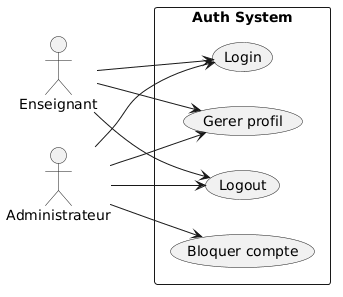
\includegraphics[width=0.7\textwidth]{images/01.png}


\section{Gestion du catalogue de mat\'eriels et des cat\'egories}

\textbf{R\^ole :} Cette fonctionnalit\'e permet \`a l'administrateur de
maintenir un inventaire structur\'e et \`a jour du mat\'eriel p\'edagogique
disponible au sein du d\'epartement.

\textbf{Fonctionnement :} Les mat\'eriels sont organis\'es en cat\'egories
(projecteurs, capteurs, mat\'eriels de TP, marqueurs, etc.). Pour chaque
mat\'eriel, l'administrateur renseigne un nom, une cat\'egorie, un \'etat
(disponible, en cours d'utilisation, en panne, en maintenance) et une
description optionnelle. L'\'etat du mat\'eriel est mis \`a jour
automatiquement lors des pr\^ets et des retours, mais peut aussi \^etre
modifi\'e manuellement. La suppression d'un mat\'eriel est logique
(soft delete) : les donn\'ees historiques sont pr\'eserv\'ees. La
suppression d'une cat\'egorie est bloqu\'ee si des mat\'eriels lui sont
encore rattach\'es.

\textbf{Exp\'erience utilisateur :} L'administrateur dispose d'un tableau
de gestion avec filtres par nom, cat\'egorie et \'etat. Des badges color\'es
indiquent visuellement l'\'etat de chaque mat\'eriel. L'ajout et la
modification se font via des formulaires intuitifs avec validation en
temps r\'eel.

\textbf{Exemple d'utilisation :} L'administrateur ajoute un nouveau
projecteur re\c{c}u par le d\'epartement, le classe dans la cat\'egorie
<<\,Vid\'eoprojection\,>> et lui attribue le statut <<\,Disponible\,>>.

	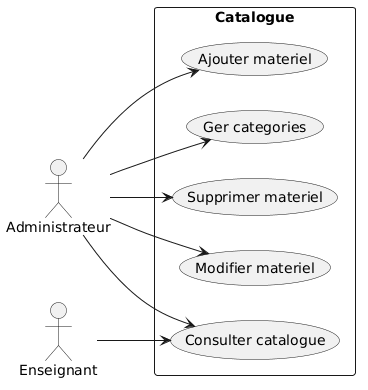
\includegraphics[width=0.7\textwidth]{images/02.png}


\section{R\'eservation de mat\'eriel par les enseignants}

\textbf{R\^ole :} Cette fonctionnalit\'e est le c\oe ur op\'erationnel
de l'application du point de vue des enseignants. Elle leur permet de
soumettre des demandes de pr\^et pour une p\'eriode donn\'ee.

\textbf{Fonctionnement :} L'enseignant s\'electionne une date de d\'ebut
et une date de fin, puis consulte les mat\'eriels disponibles sur cette
p\'eriode gr\^ace \`a un service de v\'erification automatique des
conflits. Si des mat\'eriels sont disponibles, il soumet sa demande,
enregistr\'ee avec le statut <<\,en attente\,>>. Une notification est
imm\'ediatement envoy\'ee \`a l'administrateur. L'acc\`es \`a cette
fonctionnalit\'e est refus\'e aux comptes bloqu\'es.

\textbf{Exp\'erience utilisateur :} L'interface propose un double
s\'electeur de dates avec validation c\^ot\'e client. Un bouton
<<\,V\'erifier la disponibilit\'e\,>> affiche en temps r\'eel les
mat\'eriels libres sur la p\'eriode choisie. Une fen\^etre de confirmation
r\'ecapitulative est pr\'esent\'ee avant la soumission finale.

\textbf{Exemple d'utilisation :} Un enseignant pr\'epare une s\'eance de
TP pour la semaine suivante. Il v\'erifie les capteurs disponibles du
15 au 17 novembre, constate que trois unit\'es sont libres et soumet sa
demande. Il re\c{c}oit un accus\'e de r\'eception par e-mail.

	
	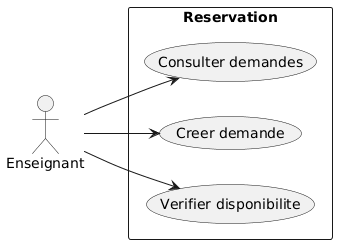
\includegraphics[width=0.7\textwidth]{images/03.png}


\section{Validation et gestion des r\'eservations par l'administrateur}

\textbf{R\^ole :} Cette fonctionnalit\'e donne \`a l'administrateur le
contr\^ole total sur le flux des demandes de r\'eservation, depuis leur
r\'eception jusqu'\`a leur traitement.

\textbf{Fonctionnement :} L'administrateur acc\`ede \`a une liste pagin\'ee
et filtr\'ee de toutes les demandes. Pour valider une demande, il
s\'electionne parmi les mat\'eriels disponibles sur la p\'eriode concern\'ee
celui qu'il souhaite affecter. Le statut de la r\'eservation passe \`a
<<\,valid\'ee\,>> et le mat\'eriel est automatiquement marqu\'e comme
<<\,en cours d'utilisation\,>>. En cas de rejet, l'administrateur peut
indiquer une raison, et l'enseignant en est notifi\'e. Les demandes en
attente sont mises en \'evidence visuellement pour une prise en charge
rapide.

\textbf{Exp\'erience utilisateur :} Un tableau de bord synth\'etique met
en avant les demandes urgentes. Chaque ligne propose des boutons d'action
directs (Valider, Rejeter, Voir). La validation s'effectue via un panneau
guid\'e en quelques clics.

\textbf{Exemple d'utilisation :} L'administrateur re\c{c}oit une notification
SMS signalant une nouvelle demande. Il se connecte, s\'electionne un
projecteur disponible et confirme la validation. L'enseignant re\c{c}oit
instantan\'ement un e-mail de confirmation.

	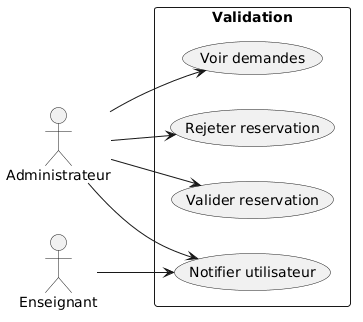
\includegraphics[width=0.7\textwidth]{images/04.png}


\section{Suivi des pr\^ets et enregistrement des retours}

\textbf{R\^ole :} Ce module garantit la tra\c{c}abilit\'e compl\`ete de
chaque \'equipement pr\^et\'e, depuis sa sortie du stock jusqu'\`a son
retour et l'\'evaluation de son \'etat.

\textbf{Fonctionnement :} \`A chaque pr\^et, l'administrateur enregistre
l'enseignant b\'en\'eficiaire, le mat\'eriel concern\'e, la date de pr\^et
et la date de retour pr\'evue. Lors du retour, il renseigne la date
effective et l'\'etat du mat\'eriel (bon \'etat, endommag\'e, perdu).
En cas de dommage, l'\'etat du mat\'eriel est automatiquement mis \`a jour.
Les pr\^ets en retard sont automatiquement signal\'es. L'historique des
pr\^ets est immuable : aucune modification ou suppression n'est autoris\'ee,
garantissant l'int\'egrit\'e de la tra\c{c}abilit\'e.

\textbf{Exp\'erience utilisateur :} La liste des pr\^ets actifs est
organis\'ee en onglets (en cours, en retard, tous). Les pr\^ets d\'epassant
leur date de retour pr\'evue sont signal\'es par un badge rouge.
L'enregistrement d'un retour s'effectue via une fen\^etre modale rapide.

\textbf{Exemple d'utilisation :} Un enseignant ram\`ene un capteur avec
un jour de retard. L'administrateur ouvre le dossier de pr\^et, enregistre
le retour en s\'electionnant l'\'etat <<\,bon \'etat\,>>. Le capteur
repasse automatiquement en statut <<\,disponible\,>>.

	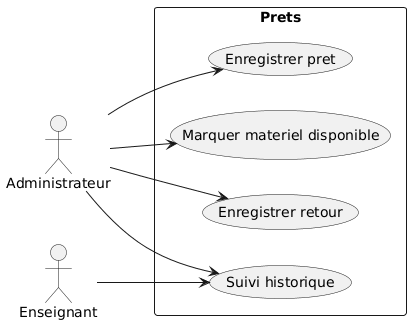
\includegraphics[width=0.7\textwidth]{images/05.png}

\section{Statistiques et tableaux de bord}

\textbf{R\^ole :} Cette fonctionnalit\'e offre \`a l'administrateur une
vision analytique de l'utilisation du parc mat\'eriel, facilitant la prise
de d\'ecisions en mati\`ere de gestion et d'investissement.

\textbf{Fonctionnement :} Le tableau de bord agr\`ege des indicateurs cl\'es
de performance : nombre de pr\^ets actifs, taux de disponibilit\'e global,
mat\'eriels endommag\'es sur le mois courant, pr\^ets en retard. Des
graphiques dynamiques illustrent les tendances sur 12 mois glissants, le
classement des mat\'eriels les plus utilis\'es et la r\'epartition des
pr\^ets par cat\'egorie.

\textbf{Exp\'erience utilisateur :} Des cartes KPI pr\'esentent les
indicateurs en un coup d'\oe il. Un graphique en barres visualise
l'\'evolution mensuelle des pr\^ets. Un diagramme circulaire illustre
la r\'epartition par cat\'egorie. Un s\'electeur de p\'eriode permet de
filtrer les donn\'ees par ann\'ee ou par mois.

\textbf{Exemple d'utilisation :} En fin d'ann\'ee, l'administrateur
consulte le tableau de bord pour identifier les mat\'eriels les plus
sollicit\'es et pr\'epare un rapport de renouvellement du parc \`a
destination de la direction du d\'epartement.

	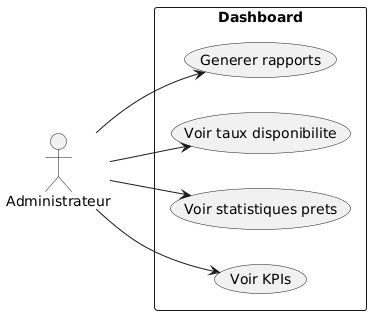
\includegraphics[width=0.7\textwidth]{images/06.png}

\chapter{Technologies et outils utilis\'es}

La r\'ealisation de ce projet mobilise un ensemble de technologies
modernes et \'eprouv\'ees dans le domaine du d\'eveloppement web.


\vspace{0.4cm}
\begin{tcolorbox}[colback=grisc,colframe=bleu!50,arc=4pt]
\begin{tabularx}{\textwidth}{>{\bfseries}p{3.4cm} X p{3.6cm}}
\toprule
\textbf{Domaine} & \textbf{Technologie / Outil} & \textbf{R\^ole} \\
\midrule
Frontend & HTML CSS JS & Interface utilisateur r\'eactive \\[0.15cm]
Backend &  Laravel (PHP) & API REST, logique m\'etier \\[0.15cm]
Base de donn\'ees &  MySQL  & Stockage des donn\'ees \\[0.15cm]
Authentification & Laravel Sanctum & Tokens d'acc\`es s\'ecuris\'es \\[0.15cm]
Notifications Email &  SMTP (sendgrid)  & E-mails transactionnels \\[0.15cm]
Notifications SMS & Twilio  & Envoi de SMS \\[0.15cm]

Environnement dev. &  Docker  & Environnement local \\[0.15cm]
H\'ebergement & Railway & D\'eploiement production \\[0.15cm]
Outils de test &  Postman  & Test des endpoints API \\[0.15cm]
\'Editeur de code &  VS Code  & D\'eveloppement \\
\bottomrule
\end{tabularx}
\end{tcolorbox}
\chapter{Perspectives et am\'eliorations futures}

L'application GestMat-DMI, dans sa version actuelle, r\'epond aux besoins
fondamentaux du d\'epartement. Toutefois, plusieurs axes d'am\'elioration
et d'\'evolution sont envisageables \`a moyen et long terme.

\section{Am\'eliorations fonctionnelles}

\textbf{R\'eservations r\'ecurrentes :} Introduire des r\'eservations
r\'ecurrentes (hebdomadaires ou mensuelles) pour les enseignants dont les
cours se tiennent de mani\`ere r\'eguli\`ere, r\'eduisant ainsi la charge
administrative li\'ee aux demandes r\'ep\'etitives.

\textbf{Annulation par l'enseignant :} Permettre \`a un enseignant
d'annuler lui-m\^eme une r\'eservation valid\'ee (sous condition de d\'elai),
lib\'erant ainsi le mat\'eriel pour d'autres utilisateurs sans intervention
de l'administrateur.

\textbf{Gestion des quantit\'es :} \'Etendre le mod\`ele de donn\'ees pour
g\'erer des \'equipements disponibles en plusieurs exemplaires, permettant
des r\'eservations partielles et une meilleure optimisation des ressources.

\section{Am\'eliorations techniques}

\textbf{Application mobile :} Le backend \'etant construit sur une API
REST d\'ecouple\'e, le d\'eveloppement d'une application mobile
(Android/iOS) serait naturellement possible sans refonte de l'architecture
serveur, am\'eliorant consid\'erablement l'accessibilit\'e pour les
enseignants.

\textbf{Exportation de rapports :} Ajouter des fonctionnalit\'es
d'exportation des statistiques et de l'historique des pr\^ets au format
PDF ou Excel, pour faciliter le reporting aupr\`es de la direction du
d\'epartement.

\textbf{Authentification SSO :} Int\'egrer l'authentification unique
(\textit{Single Sign-On}) avec le syst\`eme d'information de l'universit\'e,
permettant aux utilisateurs de se connecter avec leurs identifiants
institutionnels.

\chapter{Conclusion}

Ce projet a permis de concevoir et de d\'evelopper une application web
compl\`ete r\'epondant \`a un besoin r\'eel et concret du D\'epartement
de Math\'ematiques et Informatique de l'Universit\'e de Ngaound\'er\'e :
la gestion num\'erique et centralis\'ee du mat\'eriel p\'edagogique.

\`A travers ce travail, l'ensemble des objectifs fix\'es a \'et\'e
atteint. Un syst\`eme d'authentification s\'ecuris\'e \`a double r\^ole
a \'et\'e mis en place, garantissant un acc\`es contr\^ol\'e et adapt\'e
\`a chaque type d'utilisateur. Un catalogue structur\'e de mat\'eriels et
de cat\'egories offre une visibilit\'e en temps r\'eel sur l'\'etat du parc
mat\'eriel. Le syst\`eme de r\'eservation, coupl\'e \`a un service de
v\'erification automatique des conflits de disponibilit\'e, simplifie
consid\'erablement le processus de demande pour les enseignants. Le module
de validation administrative assure un contr\^ole rigoureux des
affectations, tandis que le suivi des pr\^ets garantit une tra\c{c}abilit\'e
totale et permanente. Enfin, le tableau de bord statistique fournit \`a
l'administration des outils d'aide \`a la d\'ecision fond\'es sur des
donn\'ees objectives.

Sur le plan p\'edagogique, ce projet a \'et\'e l'occasion de mettre en
pratique de nombreuses comp\'etences acquises au cours de la formation :
la mod\'elisation relationnelle de bases de donn\'ees, l'architecture
d'une API REST s\'ecuris\'ee, la conception d'interfaces utilisateur
r\'eactives, la mise en {\oe}uvre de bonnes pratiques de s\'ecurit\'e web,
et le travail collaboratif en \'equipe sur un projet logiciel d'envergure.

Les b\'en\'efices attendus sont multiples : gain de temps pour les
enseignants et les administrateurs, r\'eduction des conflits de
disponibilit\'e, meilleure pr\'eservation et tra\c{c}abilit\'e du
mat\'eriel, et prise de d\'ecision facilit\'ee gr\^ace aux donn\'ees
analytiques. \`A terme, ce projet pourrait constituer un mod\`ele
r\'eplicable pour d'autres structures de l'universit\'e, contribuant ainsi
\`a la modernisation progressive des processus administratifs de
l'enseignement sup\'erieur au Cameroun.



\end{document}
